\subsection{Einführung}

\begin{beispiel}
$z = \frac{1}{1+i} = \frac{1}{2} - \frac{i}{2}$\\
$|z| = \frac{1}{\sqrt{2}}, z = \frac{1}{\sqrt{2}}(\cos(-\pi/4)+i\sin(-\pi/4))$
\end{beispiel}

\begin{lemma}
\[
(\cos\phi + i\sin\phi)(\cos\phi\prime + i\sin\phi\prime))
\]
\[ \text{mit anderen Worten } arg(z*z\prime) = arg(z)+ arg(z\prime)
\]
\end{lemma}

\begin{bew}
Additionstheorem der Winkelfunktion.
\end{bew}
\begin{bemerkung}
	Geometrische Konstruktion der komplexen Multiplikation \\
	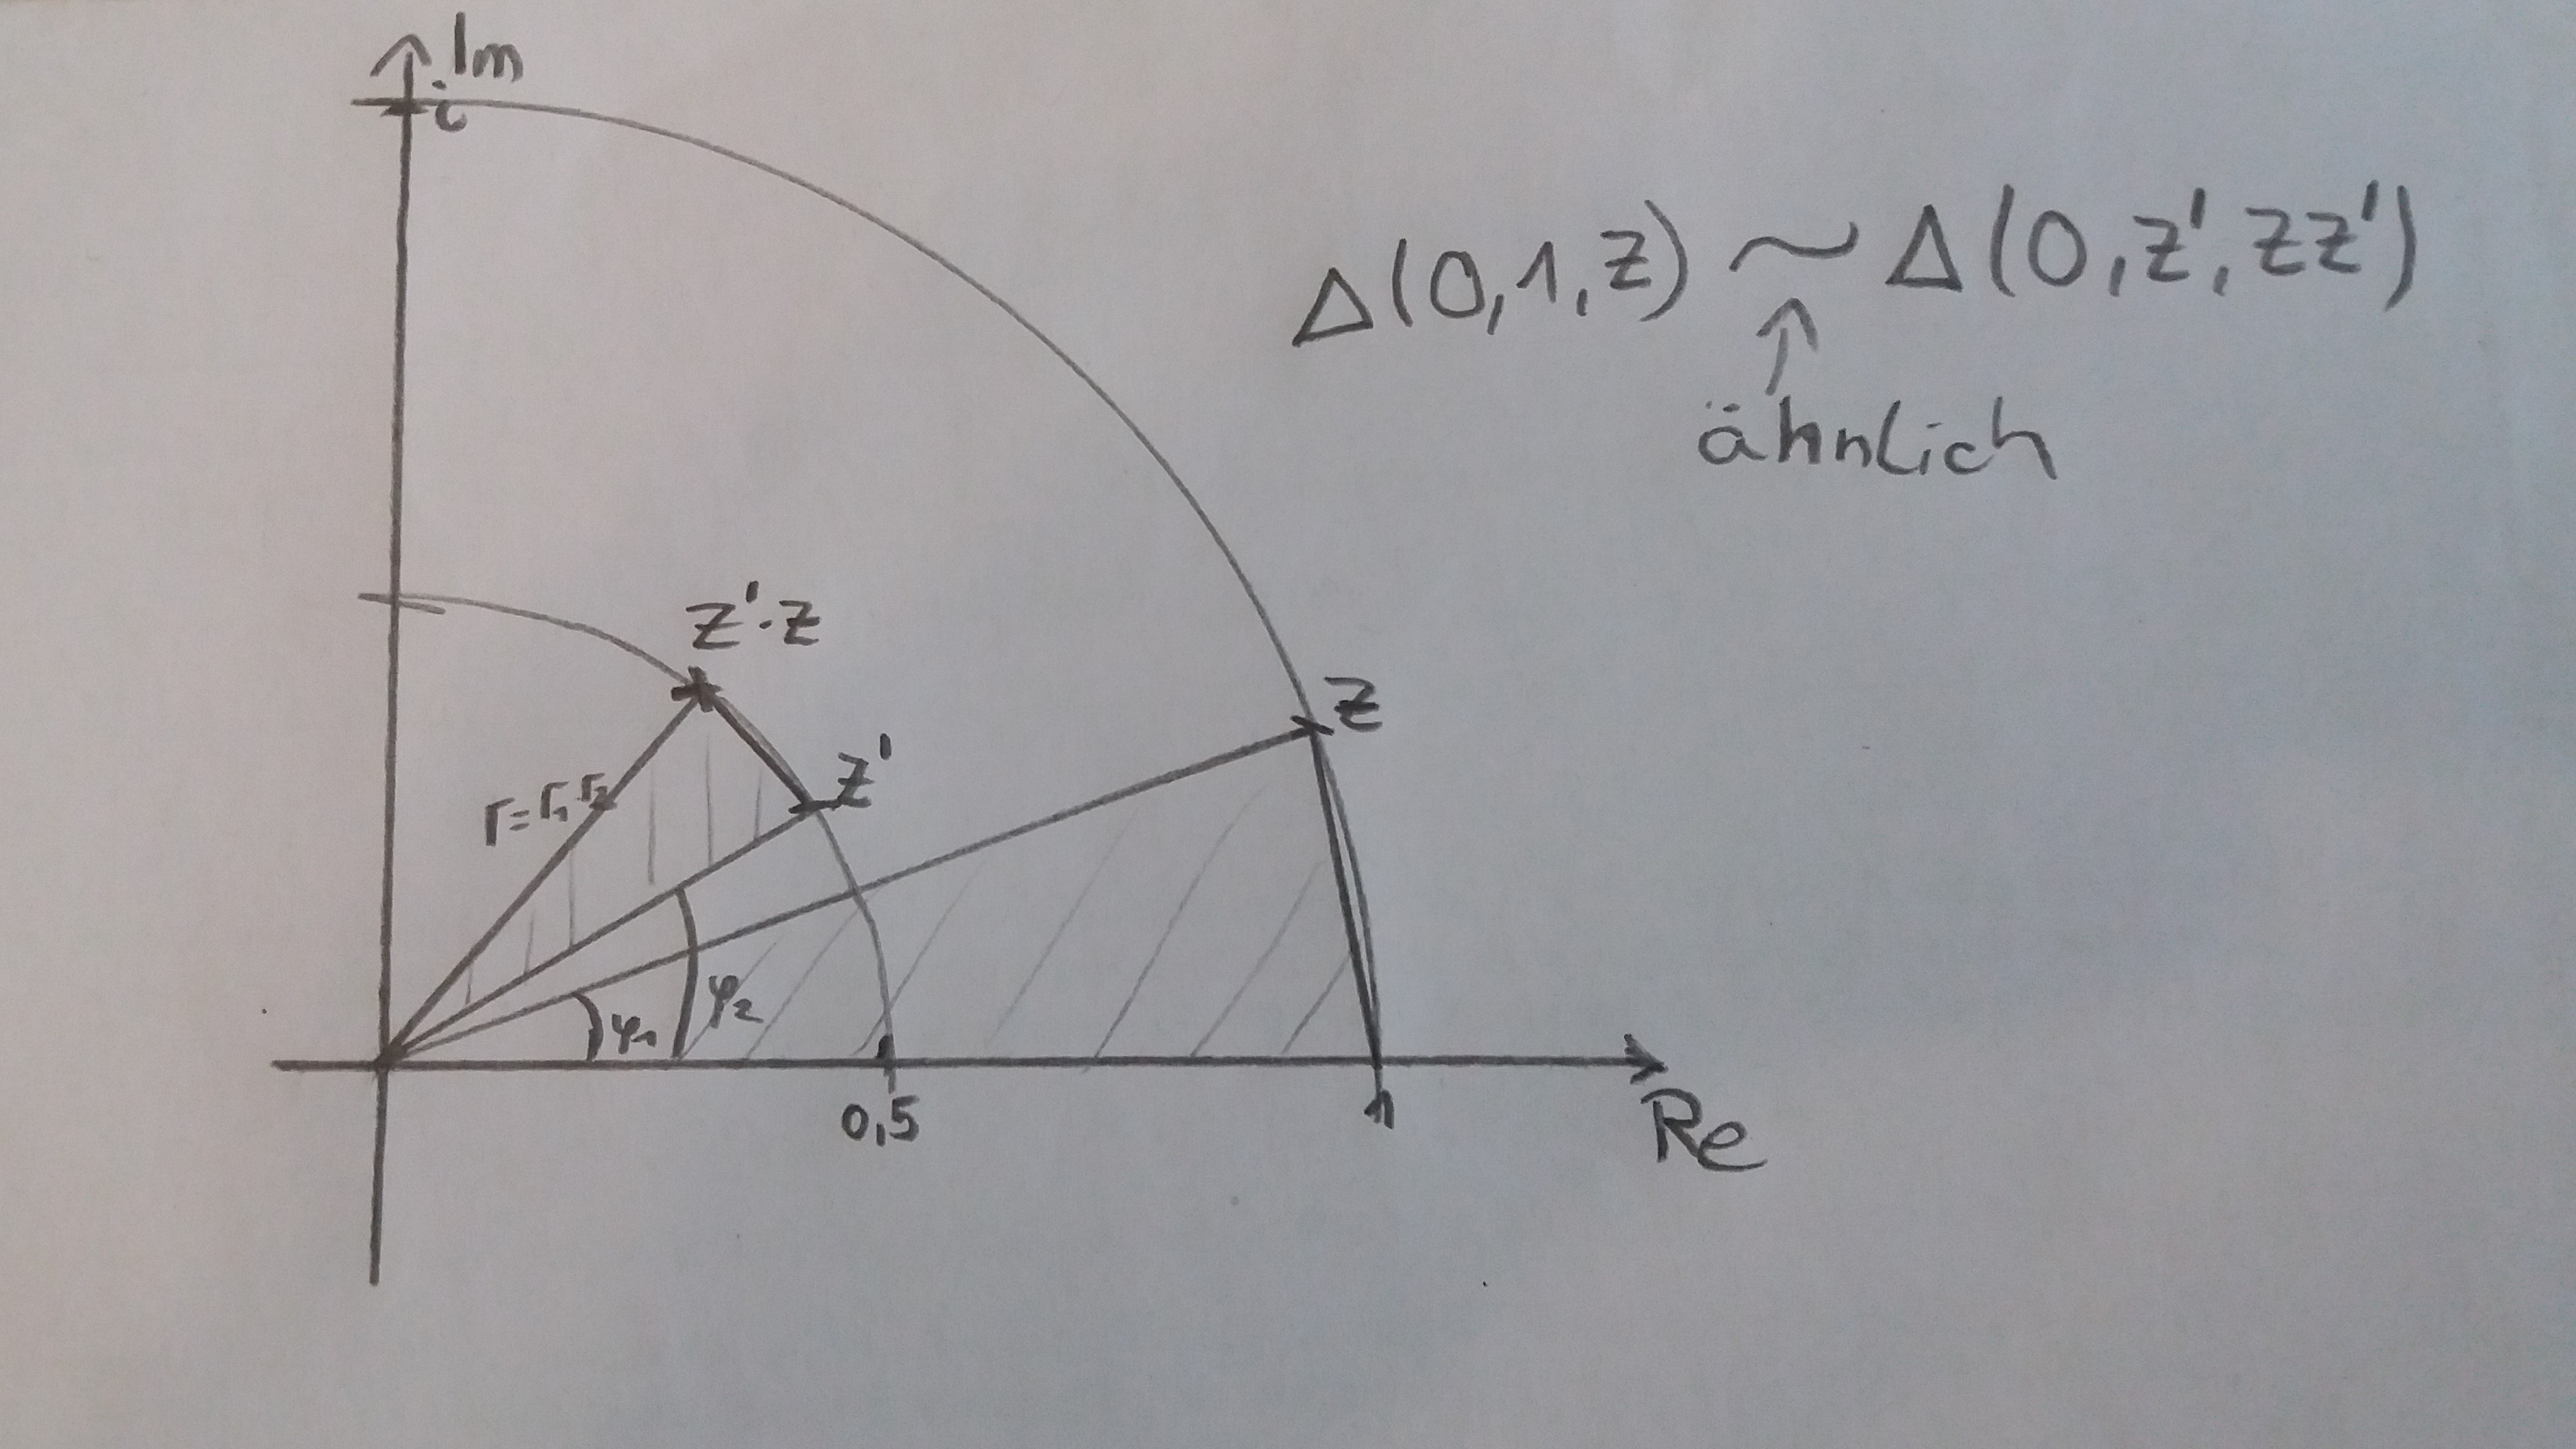
\includegraphics[scale=0.125]{pics/PolarMul.jpg} 
	Geometrische Konstruktion von $\frac{z}{z'}$ in Übungsaufgabe 8
\end{bemerkung}

\begin{definition}
$z \in \C $ heißt \textbf{m-te Einheitswurzel}, falls gilt $z^m = 1 \quad, m \in \N$ \\
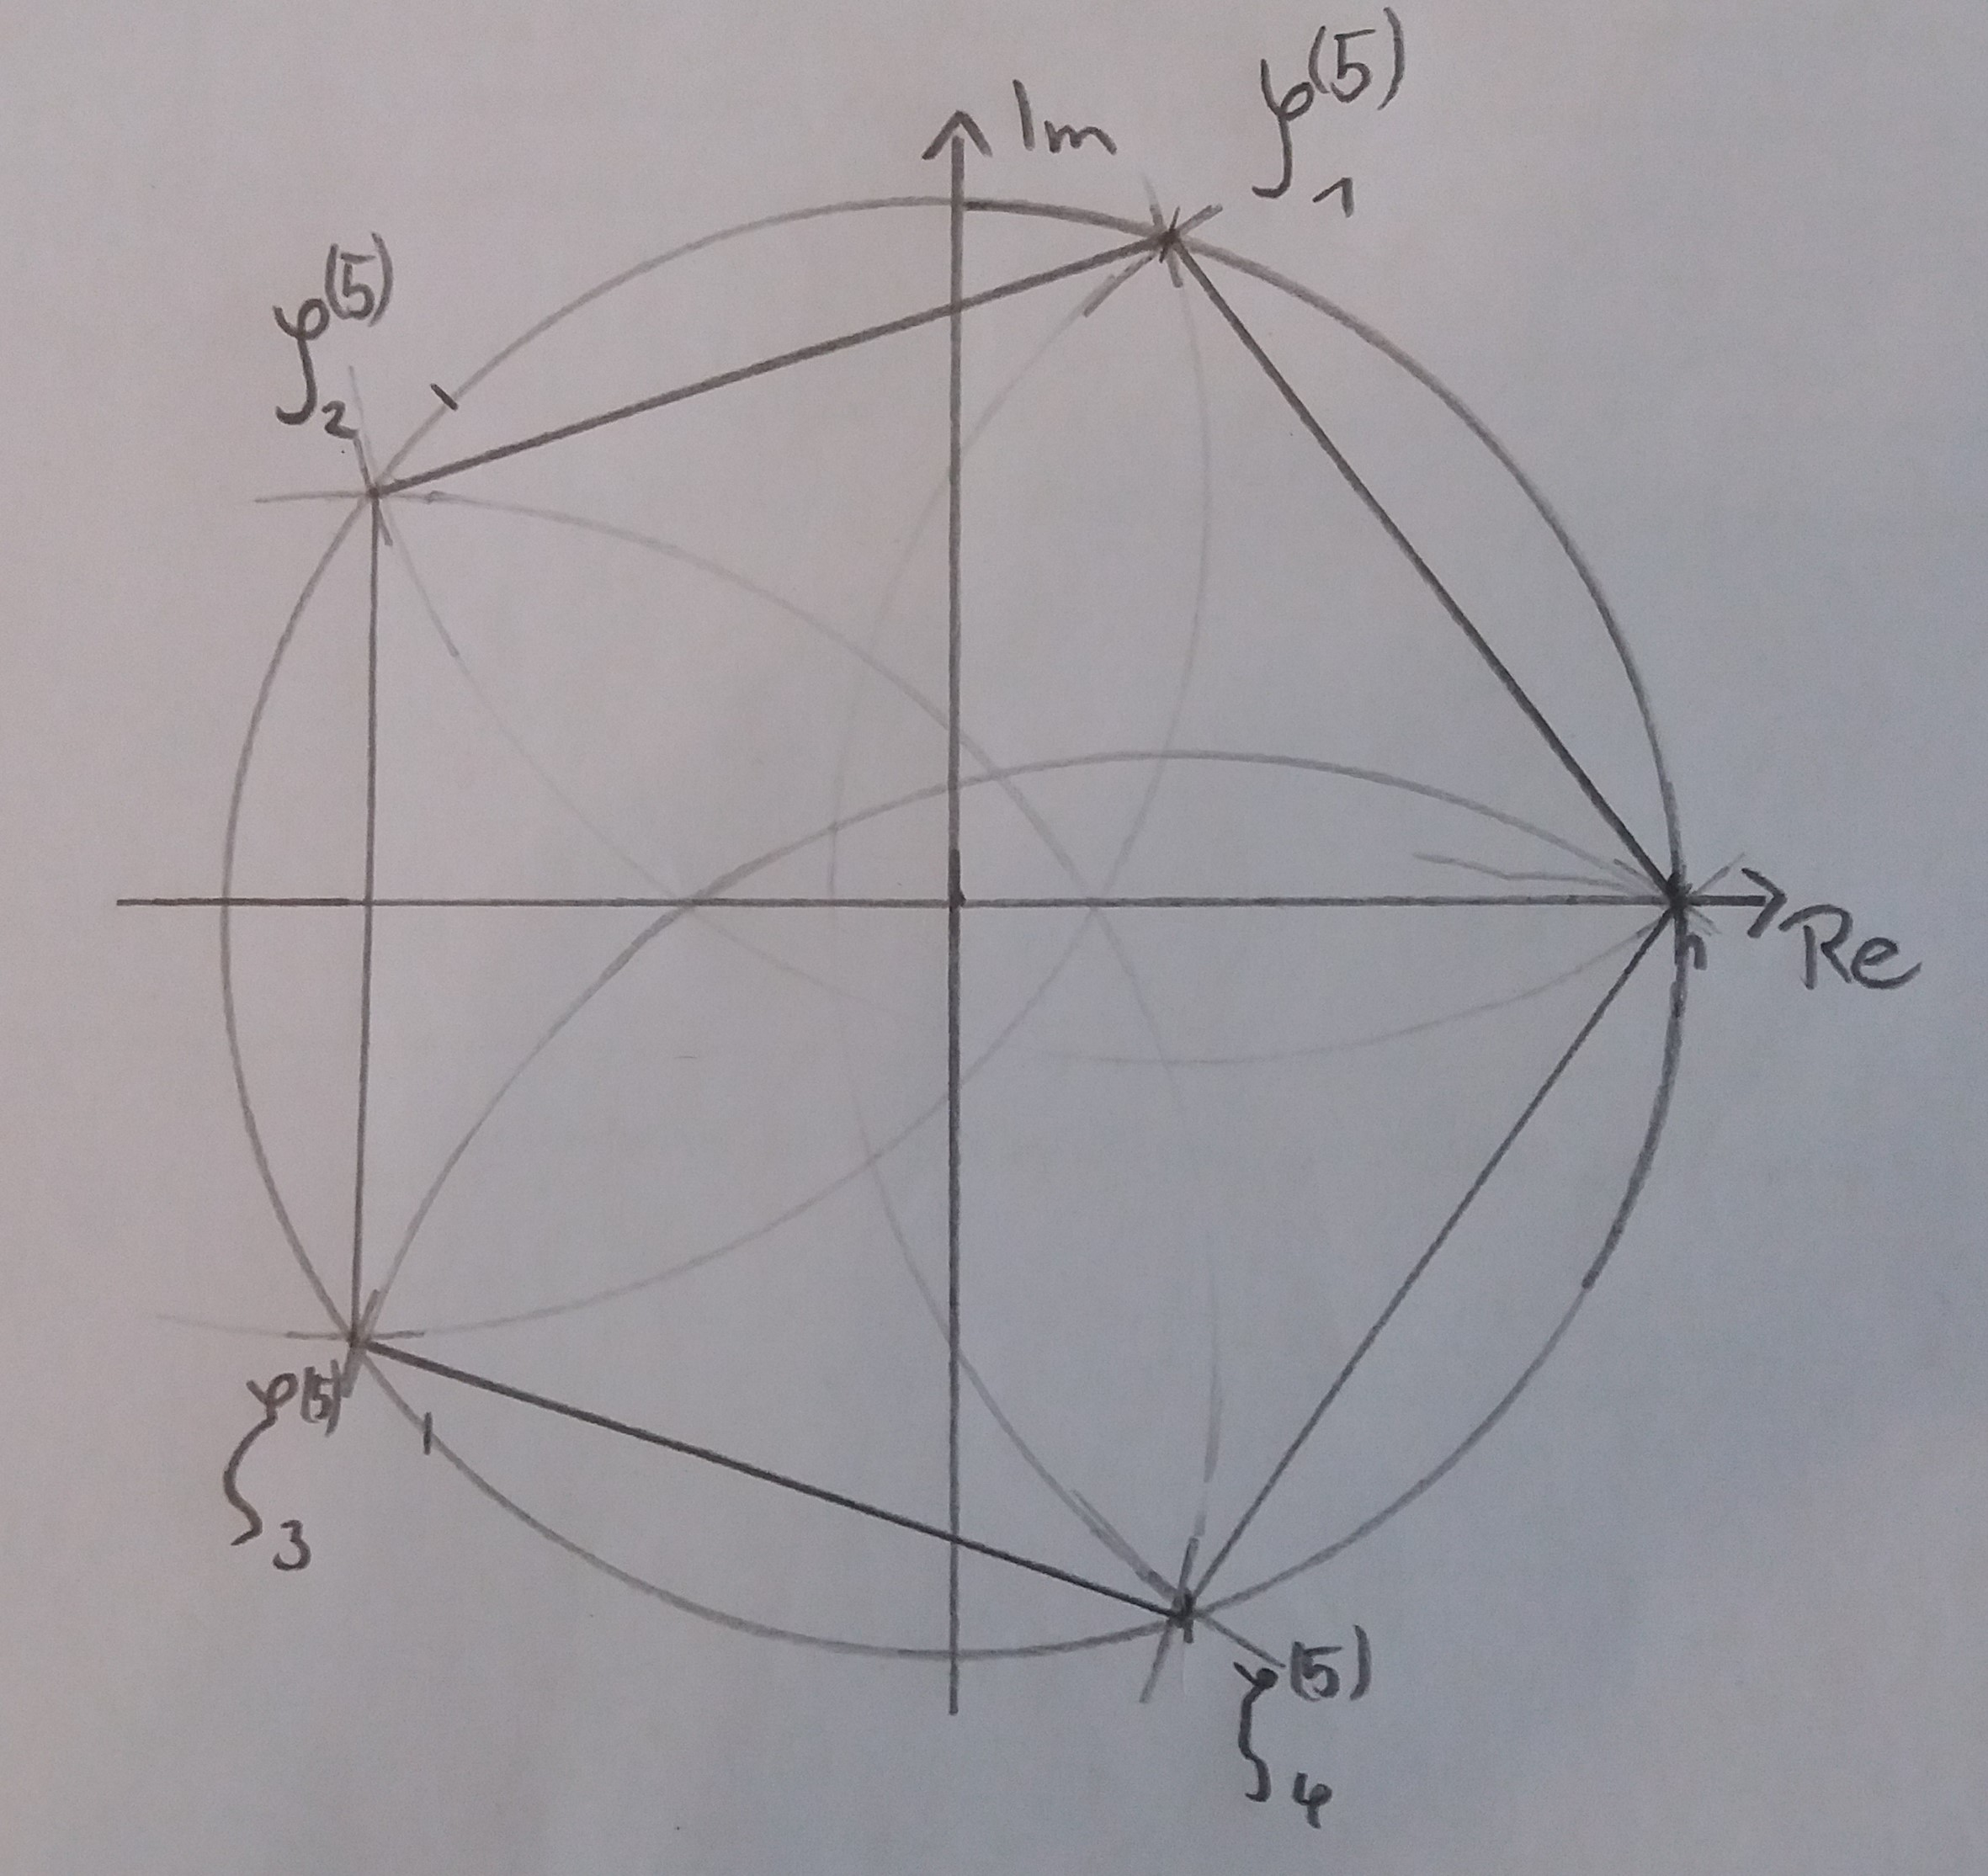
\includegraphics[scale=0.125]{pics/Wurzeln.jpg} \\
geometrische Anschauung für Einheitswurzeln als regelmäßiges Vieleck 
\end{definition}
\begin{satz}
Zu jedem $m \in \N$ gibt es genau m verschiedene m-te Einheitswurzeln:
\[
\zeta^{(m)}_k := \cos(2\pi\frac{k}{m})+i\sin(2\pi\frac{k}{m})\quad, k=0,\dots,m-1
\]
Beweis Übungsaufgabe 3.
\end{satz}

\subsection{Konvergente Folgen und Reihen}
\begin{definition}
Eine Folge $(z)_{n \in \N}, z_n \in \C$ heißt \textbf{Nullfolge}, falls $\forall \veps > 0 \quad \exists N \in \N$ mit: 
\[|z_n| < \veps \quad ,\forall n>N.\] \\
Eine Folge $(z_n)_{n\in \N}, z_n \in \C$ \textbf{konvergiert gegen z} $\in \C$
falls die Folge $(z_n-z)_{n\in \N}$ ein Nullfolge ist. Der Grenzwert ist eindeutig bestimmt: 
$\begin{displaystyle}
	z = \lim_{n \to \infty}z_n
\end{displaystyle}$
\end{definition}

\begin{bemerkung}
\leavevmode
\begin{itemize}
	\item[1)] Sei $(z_n)_{n\in\N},z_n \in \C$ eine Folge , $z \in \C$.
	\[\lim_{n\to\infty} z_n = z \Leftrightarrow (\lim_{n\to\infty}Re(z_n)=Re(z) \land\lim_{n\to\infty}Im(z_n)=Im(z)) \]
	\item[2)] Sei $(w_n)_{n\in\Z},w_n \in \C$ weitere Folge, mit $w = \lim_{n \to \infty} w_n$
	\begin{eqnarray*}
		&&\lim_{n \to \infty}(z_n \pm w_n) = z \pm w\\
		&&\lim_{n \to \infty}z_nw_n = zw\\
		&&\lim_{n \to \infty}|z_n| = |z| \\
		&&\lim_{n \to \infty}\overline{z}_n = \overline{z} \\
		&&\lim_{n \to \infty} \frac{1}{z_n}= \frac{1}{z}\quad \text{, falls } z_n \neq 0, z\neq 0
	\end{eqnarray*}
\end{itemize}
\end{bemerkung}

\begin{definition}
Sei $(z_n)_{n\in\N}, z_n \in \C$, eine Folge.\\
Die Folge der Partialsummen $(S_n)_{n\geq 0}$ mit $S_n := z_0+\dots+z_n$ heißt die der \textbf{Folge $(z_n)$ zugeordnete Reihe}.
Falls $(S_n)$ konvergiert, so heißt 
$\begin{displaystyle}
	S:=\lim_{n\to \infty} S_n
\end{displaystyle} $ Wert der Reihe und wir schreiben $\begin{displaystyle}
	\sum^\infty_{n=0}z_n := S.
\end{displaystyle}$\\
Eine Reihe 
$\begin{displaystyle}
\sum^\infty_{n=0} z_n
\end{displaystyle}$ heißt \textbf{absolut konvergent} falls die Reihe 
$\begin{displaystyle}
\sum^\infty_{n=0} |z_n|
\end{displaystyle}$ konvergiert.
\end{definition}

\begin{beispiel}
Die geometrische Reihe konvergiert für alle $z \in \C$ zu
$\begin{displaystyle}
	\sum_{\infty}^{n=0} z^n = \frac{1}{1-z}
\end{displaystyle}$
, falls $|z| <  1$ divergiert für $|z| \ge 1$
\end{beispiel}
\begin{bew}
	Es gilt: 
	$\begin{displaystyle}
	\sum_{n=0}^{N} z^n = \frac{1- z^{N+1}}{1-z}\\
	\lim_{n \to \infty} z^n = 0
	\end{displaystyle}$, falls $|z| > 1 \text{ und } |z^n| \ge 1 \text{ falls } |z| \ge 1$
\end{bew}

\begin{satz}
Eine absolut konvergente Reihe konvergiert.
\end{satz}
\begin{bew}
Analysis 1 und Bemerkung 2.2.1
\end{bew}

\begin{definition}
Da die Reihe
\[
\sum^\infty_{n=0} \frac{z^n}{n!}, \sum^\infty_{n=0} \frac{(-1)^n z^{2n}}{(2n)!}, \sum^\infty_{n=0} \frac{(-1)^nz^{2n+1}}{(2n+1)!}
\]
absolut konvergent für alle $z \in \C$ definieren wir: \\
\begin{eqnarray*}
	\exp(z) &=& \sum^\infty_{n=0} \frac{z^n}{n!} \\
	\cos(z) &=& \sum^\infty_{n=0} \frac{(-1)^n z^{2n}}{(2n)!} \\
	\sin(z) &=& \sum^\infty_{n=0} \frac{(-1)^nz^{2n+1}}{(2n+1)!}
\end{eqnarray*}
\end{definition}

\begin{lemma}[Multiplikationssatz von Cauchy]

Seien $\begin{displaystyle}
\sum^\infty_{n=0} z_n \quad ,\sum^\infty_{m=0} w_m
\end{displaystyle}$ absolut konvergente Reihen dann gilt:
\[
(\sum^\infty_{n=0} z_n)(\sum^\infty_{m=0} w_m) = \sum^\infty_{n=0} \sum^n_{k=0} z_k w_{n-k}
\]
und die rechte Seite ist ebenfalls absolut konvergent.
\end{lemma}
\begin{bew}
Kopie des Bew. aus Analysis 1
\end{bew}

\begin{satz}
\[
\exp(z) \exp(w) = \exp(z+w)\quad \forall z,w \in \C
\]
\end{satz}
\begin{bew}
\[
\sum \frac{z^n}{n!} \sum \frac{w^m}{m!} = \sum \sum \frac{z^kw-k}{n!(n-k)!} = \sum \frac{(z+w)^n}{n!}
\]
\end{bew}

\begin{korollar}\label{korollar1}
	\begin{eqnarray*}
		\exp(z) &\neq& 0\\
		\exp(z)^n &=& \exp(nz)\\
		\exp(iz) &=& \cos(z) + i \sin(z)\\
		\cos(z) &=& \frac{1}{2} (\exp(iz)+\exp(-iz))\\
		\sin(z) &=& \frac{1}{2i} (\exp(iz)-\exp(-iz))\\
		\text{sei z = x + iy, } \exp z &=& e^x ( \cos(y) + i \sin(y)) \\
		|\exp(z) | &=& e^x\\
		\cos(z+w) &=& \cos(z)\cos(w) - \sin(z) \sin(w)\\
		\sin(z+w) &=& \cos(z) \sin(w) + \sin(z) \cos(w)
	\end{eqnarray*}
\end{korollar}

\begin{bemerkung}\label{bemerkung1}
$\exp(z)$ ist nicht injektiv, da $\exp(2\pi i k ) = 1 \quad\forall k \in \Z$.\\
Genauer $ \exp(z) = \exp(w) \Leftrightarrow z-w \in 2\pi i \Z$ \\
also $ker( \exp) = \{z \in \C| \exp(z) = 1\} = 2\pi i \Z$ \\
\[\exp( z+w) = \exp( z) \quad\forall z \in \C \Leftrightarrow w \in ker (\exp).\]\\
Die Exponentialfunktion \textbf{ist periodisch} mit Perioden $2 \pi i k, k \in \Z$.\\
\begin{eqnarray*}
	\sin z = 0 &\Leftrightarrow & z = k\pi, k \in \Z \\
	\cos z = 0 &\Leftrightarrow & z = (k+ 1/2)\pi, k \in \Z
\end{eqnarray*}
\end{bemerkung}

Sei
$ S = \{ w \in \C| -\pi < Im(w) \leq \pi\}$\\
$\exp|_S$ ist injektiv, wegen Periodizität
\begin{eqnarray*}
	\{\exp(z)| z \in S\} = \{ \exp(z) | z \in \C\}\\
	\Rightarrow \{ \exp(z) | z \in \C \} = \C^{\times}\\
	\exp|_S: S \to \C^{\times}\\
	z \mapsto \exp (z) \text{ ist bijektiv}
\end{eqnarray*}

\begin{definition}
Wegen Bemerkung \ref{bemerkung1} existiert eine eindeutig bestimmte Zahl $w\in S \text{ mit } \exp(w)= z$. w heißt \textbf{Hauptwert des Logarithmus von z} und wir schreiben $w = Log(z) $
\end{definition}
\begin{satz}
	\leavevmode
\begin{itemize}
	\item[1)]
	Es existiert eine Funktion, der sogenannte \textbf{Hauptzweig des Log}, $ Log: \C^{\times} \to \C$ , welche durch $ \exp(Log(z)) = z \text{ und } -\pi< Im(Log (z)) \leq \pi$ eindeutig bestimmt ist.
	\item[2)]
	$\exp (w) = z \Rightarrow w = Log( z) + 2 \pi i , k \in \Z$
	\item[3)]
	$Log (z) = \log (z)$ falls $ z \in \R^{\times}_+$
	\item[4)]
	$Log (z) = \log(|z|) + i Arg(z)$
\end{itemize}
\end{satz}
\begin{bew}
1) folgt aus Bemerkung \ref{bemerkung1}, ebenso 2) aus 1) und Bem. \ref{bemerkung1}, 3) klar, 4) folgt aus 1),Korollar \ref{korollar1} und ?1.8?
\end{bew}